    \documentclass[11pt]{article}

    \usepackage[utf8]{inputenc}
    \usepackage[T1]{fontenc}
    \usepackage[brazilian]{babel}
    \usepackage[a4paper,margin=2.5cm]{geometry}
    \usepackage{graphicx}
    \graphicspath{{latex_figures/}}
    \usepackage{booktabs}
    \usepackage{caption}
    \usepackage{float}
    \usepackage{hyperref}

    \title{Segmentação Automática de B-Lines em Ultrassom Pulmonar: \\
    Comparação de Arquiteturas e Representações de Saída}
    \author{}
    \date{28 de setembro de 2026}

    \begin{document}

    \maketitle

    % ============================================================
    \section{Contexto e Objetivo}
    % ============================================================

    O projeto estuda a segmentação automática de B-Lines em ultrassom pulmonar. A ideia
    central não é apenas treinar um modelo, mas montar uma estrutura de experimentos que
    permita comparar representações geométricas no mesmo dataset e split, registrando
    as diferenças de framework, augmentation, checkpoint selection e avaliação.

    As anotações originais estão no formato YOLO Polygon: cada B-Line é um quadrilátero
    de 4 vértices (classe $x_1\ y_1\ x_2\ y_2\ x_3\ y_3\ x_4\ y_4$, coordenadas
    normalizadas).

    % ============================================================
    \section{Dataset}
    % ============================================================

    O conjunto de treino tem 256 imagens. O conjunto de validação tem 75 imagens e 115
    instâncias anotadas (1,53 B-Lines por imagem, em média). Existe ainda um conjunto de
    teste com 70 imagens, mas sem rótulo até o momento.

    Como o teste não tem anotação, todos os números reportados neste trabalho vêm do
    conjunto de validação --- o mesmo usado para acompanhar o treino. Isso é discutido
    na Seção~\ref{sec:limitacoes} como limitação.

    % ============================================================
    \section{Protocolo Experimental}
    % ============================================================

    Mask R-CNN, Faster R-CNN e Polygon Head usam backbone ResNet-50 com FPN e pesos
    COCO no Detectron2. As execuções históricas usaram batch de 4, taxa de aprendizado
    0,00025 e 2000 iterações, com avaliação e checkpoint a cada 100 iterações. Os
    pipelines diferem em augmentations, head e métrica de seleção; por isso, os números
    abaixo são preliminares e não representam protocolo idêntico. Um hook customizado
    calculava loss de validação.

    O YOLOv11 usa seu próprio protocolo de treino (framework Ultralytics), mas roda
    sobre os mesmos splits e é avaliado com COCOeval. Seu framework, augmentations,
    batch efetivo e seleção de checkpoint diferem dos pipelines Detectron2. O código
    atual registra seeds e configuração, avalia a Polygon Head por `segm_polygon/AP` e
    seleciona checkpoints pela métrica configurada para cada tarefa; os resultados
    históricos ainda são single-run.

    % ============================================================
    \section{Mask R-CNN (baseline)}
    \label{sec:maskrcnn}
    % ============================================================

    Arquitetura de referência do projeto: detecta a caixa delimitadora do objeto e
    prevê uma máscara binária livre, pixel a pixel, para cada instância.

    Duas observações relevantes surgiram na análise do treino. A primeira é overfitting:
    a loss de treino cai continuamente até aproximadamente 0,28, mas a loss de validação
    para de melhorar por volta da iteração 900--1400 (mínimo de 0,44) e volta a subir,
    chegando a 0,51 na iteração final (Figura~\ref{fig:mask_loss}). A segunda,
    consequência direta da primeira, é que o checkpoint final não é o melhor: o AP de
    segmentação de validação atinge seu pico na iteração 1399 (40,61) e cai para 38,33
    na iteração 2000 (Figura~\ref{fig:mask_ap}). Por isso passou-se a selecionar o
    melhor checkpoint em vez de sempre usar o último --- essa mudança sozinha elevou o
    AP de segmentação reportado de 36,7 para 40,6.

    \begin{table}[H]
    \centering
    \caption{Resultados do Mask R-CNN no melhor checkpoint (iteração 1399).}
    \begin{tabular}{lccc}
    \toprule
    Tarefa & AP & AP50 & AP75 \\
    \midrule
    Caixa delimitadora (bbox) & 54,1 & 88,8 & 57,6 \\
    Segmentação (segm) & 40,6 & 83,6 & 33,0 \\
    \bottomrule
    \end{tabular}
    \end{table}

    Na análise por instância, com matching greedy um-para-um por confiança e IoU de
    máscara de pelo menos 0,5: IoU médio de 0,52 (mediana 0,65), Dice médio de 0,61
    (mediana 0,78), precisão média de 0,59, recall médio de 0,67 e confiança média de
    0,91. No threshold otimizado na validação (0,875), o F1 chega a 0,82
    (precisão de 0,81, recall de 0,83).

    Vale registrar que, ao inspecionar as máscaras visualmente com o threshold padrão
    (0,50), apareciam máscaras borradas e detecções extras (2,31 por imagem, contra
    1,53 reais). Usando o threshold ótimo do próprio modelo, esse problema quase
    desapareceu --- parte do que parecia ``modelo ruim'' era, na verdade, visualização
    calibrada de forma inadequada. Como o threshold foi otimizado na validação, esse
    F1 é exploratório e não uma estimativa independente de generalização.

    \begin{figure}[H]
    \centering
    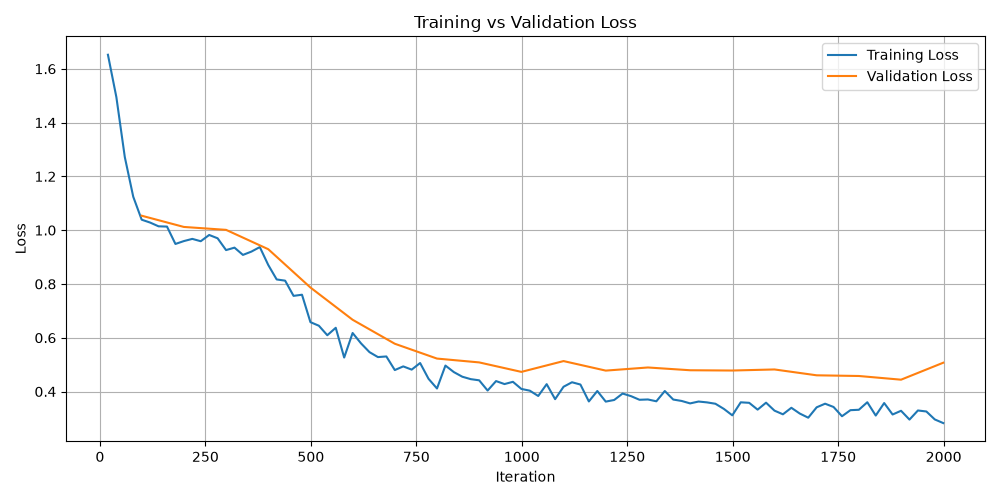
\includegraphics[width=0.8\linewidth]{mask_rcnn/train_vs_val_loss.png}
    \caption{Loss de treino vs.\ validação ao longo das 2000 iterações. A validação
    para de melhorar por volta da iteração 1000 e volta a subir no final.}
    \label{fig:mask_loss}
    \end{figure}

    \begin{figure}[H]
    \centering
    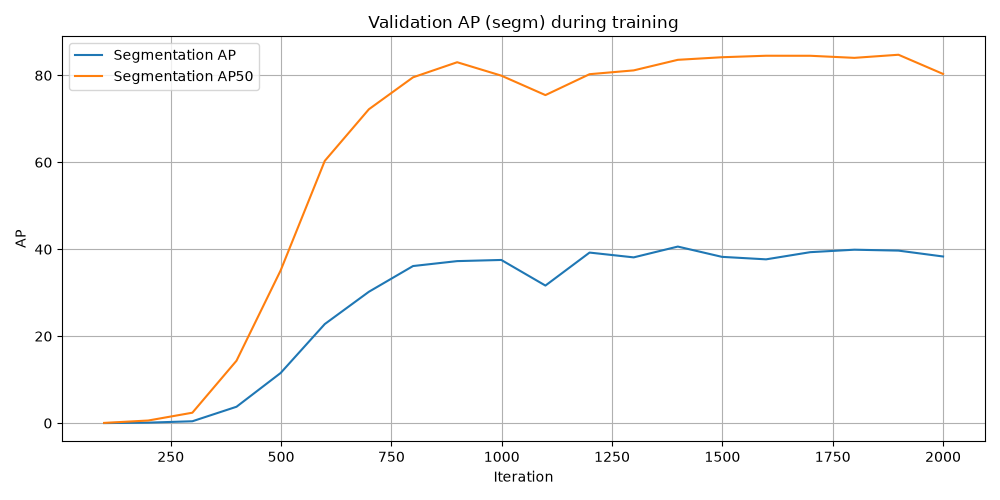
\includegraphics[width=0.8\linewidth]{mask_rcnn/val_segm_ap.png}
    \caption{AP de segmentação de validação ao longo do treino. O pico ocorre antes da
    iteração final.}
    \label{fig:mask_ap}
    \end{figure}

    \begin{figure}[H]
    \centering
    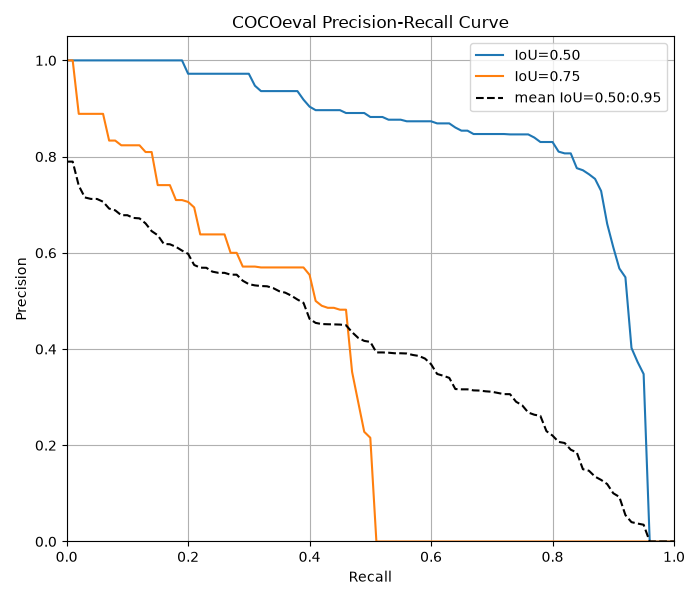
\includegraphics[width=0.8\linewidth]{mask_rcnn/coco_pr_curves.png}
    \caption{Curva Precisão--Recall oficial (COCOeval) para a tarefa de segmentação.}
    \label{fig:mask_pr}
    \end{figure}

    \begin{figure}[H]
    \centering
    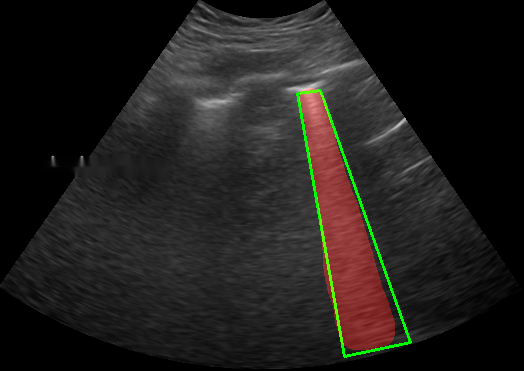
\includegraphics[width=0.6\linewidth]{predictions/mask_rcnn_1646467410642.png}
    \caption{Exemplo de predição (verde: anotação real; vermelho: máscara prevista).}
    \label{fig:mask_pred}
    \end{figure}

    % ============================================================
    \section{Faster R-CNN}
    % ============================================================

    Mesma espinha dorsal do Mask R-CNN, sem a etapa de máscara --- apenas detecta a
    caixa delimitadora. O objetivo foi isolar a dificuldade de localizar a B-Line da
    dificuldade de desenhar sua forma exata. Utiliza o mesmo dataset já registrado, sem
    nenhuma conversão adicional.

    \begin{table}[H]
    \centering
    \caption{Resultados do Faster R-CNN no melhor checkpoint.}
    \begin{tabular}{lccc}
    \toprule
    AP & AP50 & AP75 & Melhor F1 (threshold) \\
    \midrule
    54,4 & 89,1 & 59,1 & 0,85 (0,53) \\
    \bottomrule
    \end{tabular}
    \end{table}

    \begin{figure}[H]
    \centering
    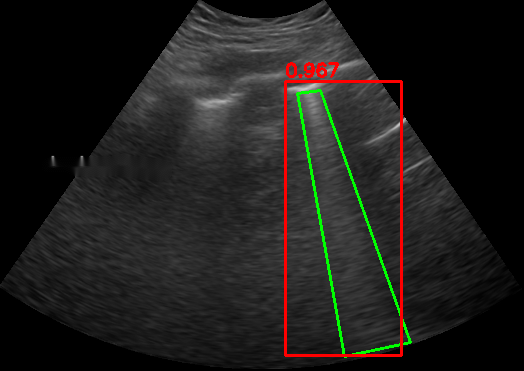
\includegraphics[width=0.6\linewidth]{predictions/faster_rcnn_1646467410642.png}
    \caption{Exemplo de predição do Faster R-CNN (verde: anotação real; vermelho: caixa
    prevista).}
    \label{fig:faster_pred}
    \end{figure}

    % ============================================================
    \section{YOLOv11}
    % ============================================================

    Arquitetura \textit{one-stage}, de família diferente da R-CNN (Ultralytics), usada
    para verificar se a dificuldade observada era específica dos modelos R-CNN.
    Utilizou-se o \texttt{yolo11n} (variante nano), com o dataset convertido de
    polígono para caixa a partir da mesma anotação original, treinado por 31 épocas ---
    equivalente ao número de imagens vistas pelo protocolo dos R-CNN (2000 iterações
    $\times$ 4 de batch / 256 imagens). Os hiperparâmetros de treino seguiram os padrões
    do Ultralytics; não foram forçados os mesmos valores do Detectron2, pois transportar
    hiperparâmetros de um framework para outro tende a prejudicar a convergência.

    As predições foram exportadas para o formato COCO e avaliadas com o mesmo código
    \texttt{pycocotools} utilizado nos demais modelos, não com a métrica nativa do
    Ultralytics, para preservar a comparação justa.

    \begin{table}[H]
    \centering
    \caption{Resultados do YOLOv11.}
    \begin{tabular}{lccc}
    \toprule
    AP & AP50 & AP75 & Melhor F1 (threshold) \\
    \midrule
    56,5 & 87,6 & 61,8 & 0,82 (0,53) \\
    \bottomrule
    \end{tabular}
    \end{table}

    \begin{figure}[H]
    \centering
    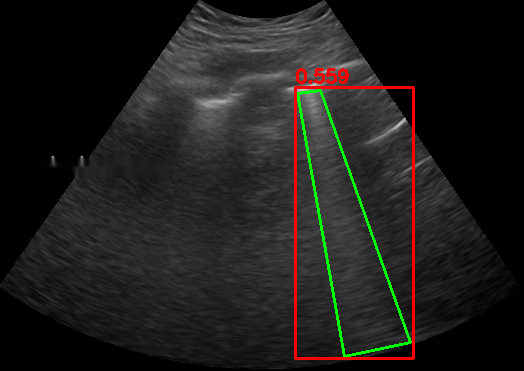
\includegraphics[width=0.6\linewidth]{predictions/yolo_1646467410642.png}
    \caption{Exemplo de predição do YOLOv11 (verde: anotação real; vermelho: caixa
    prevista).}
    \label{fig:yolo_pred}
    \end{figure}

    % ============================================================
    \section{Comparação entre os Três Modelos de Caixa}
    % ============================================================

    \begin{table}[H]
    \centering
    \caption{Comparação de AP entre Mask R-CNN (branch de caixa), Faster R-CNN e
    YOLOv11.}
    \begin{tabular}{lccc}
    \toprule
    Modelo & AP & AP50 & AP75 \\
    \midrule
    Mask R-CNN (caixa) & 54,1 & 88,8 & 57,6 \\
    Faster R-CNN & 54,4 & 89,1 & 59,1 \\
    YOLOv11 & 56,5 & 87,6 & 61,8 \\
    \bottomrule
    \end{tabular}
    \end{table}

    Os três modelos ficam num intervalo estreito, com cerca de 2,5 pontos de AP de
    diferença entre o melhor e o pior. O YOLOv11 apresenta uma vantagem discreta, mais
    visível no AP75 (localização mais precisa), mas não há diferença categórica entre
    as arquiteturas nessa tarefa.

    \begin{figure}[H]
    \centering
    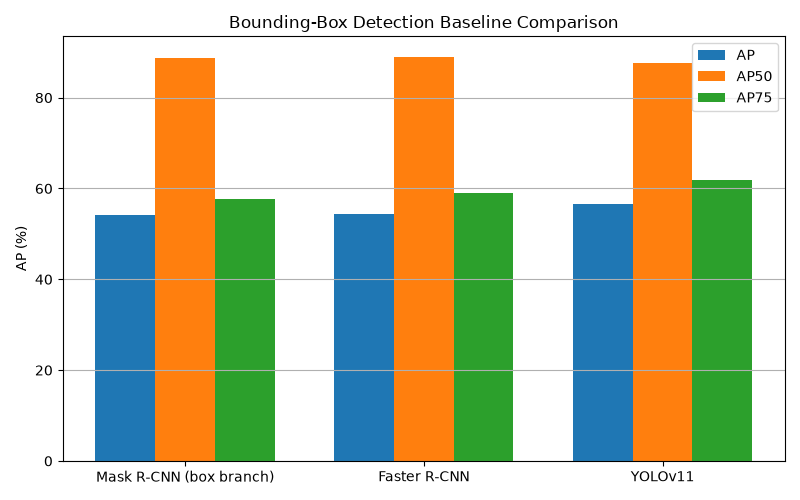
\includegraphics[width=0.7\linewidth]{comparison_ap.png}
    \caption{Comparação de AP/AP50/AP75 entre Mask R-CNN, Faster R-CNN e YOLOv11.}
    \label{fig:comparison}
    \end{figure}

    % ============================================================
    \section{Polygon Head --- Primeira Tentativa (Heatmap)}
    % ============================================================

    Em vez de uma máscara livre, a proposta da Polygon Head é prever diretamente os 4
    vértices do quadrilátero. Na primeira tentativa, reaproveitou-se a infraestrutura
    de Keypoint R-CNN já disponível no Detectron2 (originalmente concebida para pose
    humana, com 17 pontos), adaptada para 4 pontos --- cada vértice tratado como um
    ponto-chave localizado por um mapa de calor espacial. A opção por reaproveitar essa
    infraestrutura, em vez de implementar algo do zero, teve como objetivo evitar
    reimplementar, sem GPU disponível para testes interativos, as partes mais
    arriscadas: a transformação correta dos pontos quando a imagem sofre corte ou
    espelhamento durante o treino.

    \begin{table}[H]
    \centering
    \caption{Polygon Head, variante heatmap, em duas resoluções de mapa de calor.}
    \begin{tabular}{lccccc}
    \toprule
    Configuração & AP & AP50 & AP75 & Melhor F1 & \% polígono inválido \\
    \midrule
    Resolução padrão & 15,0 & 37,1 & 11,9 & 0,49 & 6,7\% \\
    Resolução dobrada & 3,8 & 10,8 & 2,7 & 0,25 & 20,4\% \\
    \bottomrule
    \end{tabular}
    \end{table}

    \noindent \textit{Polígono inválido}: os 4 vértices, conectados na ordem prevista,
    formam uma figura que se autointersecciona --- não é um quadrilátero simples.

    Aumentar a resolução do mapa de calor piorou o resultado em vez de melhorá-lo. Com
    poucos dados (256 imagens) e poucas iterações, um alvo de classificação mais fino
    é mais difícil de aprender, não mais fácil. Além disso, o heatmap trata os 4
    vértices como classificações independentes entre si --- nada na arquitetura obriga
    os pontos a formarem uma figura geometricamente coerente, o que explica a taxa de
    autointersecção observada.

    Para permitir comparação direta com o Mask R-CNN, o polígono previsto foi
    convertido de volta em uma segmentação e avaliado pelo mesmo COCOeval utilizado na
    baseline (métrica denominada \texttt{segm\_polygon}), tornando esse AP diretamente
    comparável ao AP de segmentação da Seção~\ref{sec:maskrcnn}.

    % ============================================================
    \section{Polygon Head --- Regressão Direta de Vértice}
    % ============================================================

    Diante do resultado do mapa de calor, foi implementada uma cabeça com quatro
    camadas convolucionais, \textit{pooling} global e duas camadas densas. Ela emite 8
    valores (4 vértices $\times$ 2 coordenadas) por proposta. A loss histórica é
    \textit{smooth-L1}. Esta implementação não prevê coordenadas absolutas da imagem:
    cada vértice é codificado como offset relativo ao canto superior esquerdo da
    proposta, normalizado por sua largura e altura. A nova variante centrada introduzida
    no código atual usa a mesma caixa, mas offsets relativos ao centro.

    \begin{table}[H]
    \centering
    \caption{Polygon Head, variante regressão direta, em três configurações.}
    \begin{tabular}{lccccc}
    \toprule
    Configuração & AP & AP50 & AP75 & Melhor F1 & Recall@0,5 \\
    \midrule
    Sem restrição na saída (melhor) & 12,2 & 54,2 & 1,4 & 0,63 & 0,74 \\
    Com sigmoid na saída & 4,3 & 22,9 & 0,1 & 0,37 & 0,42 \\
    Com penalidade suave de escape & 8,2 & 35,3 & 0,1 & 0,46 & 0,55 \\
    \bottomrule
    \end{tabular}
    \end{table}

    Nas três variantes, a taxa de polígono autointersectado caiu para 0\% (contra
    6,7--20,4\% do heatmap) --- a regressão direta resolve por completo esse problema
    estrutural.

    A versão sem restrição, apesar de superior às demais, produzia polígonos cerca de
    20\% maiores que o real, e 88\% das predições apresentavam algum vértice fora da
    própria caixa prevista, já que nada na arquitetura impedia isso. Duas correções
    foram testadas. A primeira, uma função sigmoide forçando a saída entre 0 e 1,
    piorou o resultado: os alvos reais concentram-se exatamente nos valores extremos
    (0 e 1, pois a caixa é definida pelos próprios vértices), e é justamente nesse
    ponto que o gradiente da sigmoide é menor --- o efeito foi travar o aprendizado em
    vez de apenas limitar a saída. A segunda, uma penalidade suave que atua somente
    quando o vértice ultrapassa o intervalo válido, também piorou o resultado, e de
    forma reveladora: a taxa de vértices fora da caixa não se alterou (permaneceu em
    torno de 88\%), evidenciando que esse comportamento nunca foi a causa do problema,
    apenas um sintoma correlacionado.

    Uma inspeção exploratória sugeriu inflação das caixas previstas. No repositório
    auditado não havia uma análise salva que quantificasse o efeito por modelo, largura,
    altura, centro, orientação, tamanho, confiança e imagem. A faixa de 12--16\% é,
    portanto, uma hipótese preliminar, não um viés confirmado em todos os detectores.
    A rotina de análise foi implementada; falta executá-la sobre predições associadas a
    checkpoints identificáveis.

    \begin{figure}[H]
    \centering
    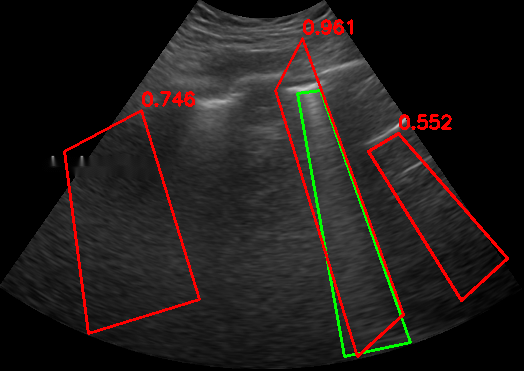
\includegraphics[width=0.6\linewidth]{predictions/polygon_head_1646467410642.png}
    \caption{Exemplo de predição da Polygon Head, regressão direta (verde: anotação
    real; vermelho: polígono previsto).}
    \label{fig:polygon_pred}
    \end{figure}

    % ============================================================
    \section{Resumo Geral}
    % ============================================================

    \begin{table}[H]
    \centering
    \caption{Comparação final entre todas as arquiteturas e representações testadas.}
    \begin{tabular}{lccc}
    \toprule
    Modelo / Representação & AP & AP50 & AP75 \\
    \midrule
    Mask R-CNN --- segmentação (máscara) & 40,6 & 83,6 & 33,0 \\
    Mask R-CNN --- caixa & 54,1 & 88,8 & 57,6 \\
    Faster R-CNN --- caixa & 54,4 & 89,1 & 59,1 \\
    YOLOv11 --- caixa & 56,5 & 87,6 & 61,8 \\
    Polygon Head heatmap (melhor variante) & 15,0 & 37,1 & 11,9 \\
    Polygon Head regressão direta (melhor) & 12,2 & 54,2 & 1,4 \\
    \bottomrule
    \end{tabular}
    \end{table}

    Nos resultados históricos, nenhuma das versões poligonais superou o Mask R-CNN com
    máscara binária livre. A regressão relativa à proposta reduz autointerseções e
    melhora AP50, recall e F1 frente ao heatmap, mas seu AP75 permanece muito baixo.
    Esses números são de execução única; ainda não demonstram estabilidade entre seeds.
    O resumo salvo no workspace corresponde à variante com penalidade (AP 8,18), não à
    variante sem restrição (AP 12,2) destacada na tabela. Assim, até reconciliar modelo,
    checkpoint e predições, a tabela deve ser lida como registro dos resultados
    históricos do relatório, e não como uma reprodução confirmada pelos artefatos locais.
    As causas possíveis incluem: a máscara herda conhecimento de pré-treino no COCO,
    enquanto a cabeça poligonal aprende a regressão
    com poucas imagens; a máscara recebe supervisão densa, enquanto a regressão usa um
    vetor compacto; e as caixas previstas podem introduzir erro na parametrização.

    % ============================================================
    \section{Auditoria do dataset, código e artefatos (28/09/2026)}
    \label{sec:auditoria}
    % ============================================================

    A inspeção local confirmou 256 imagens de treino, 75 de validação com 115 linhas de
    anotações válidas, e 70 imagens de teste sem rótulos. Todas as linhas de validação
    têm quatro vértices. No treino foram encontradas 358 linhas; duas linhas tinham
    cinco vértices: linha 2 de
    \texttt{RT\_LOWER\_LAT\_LONG-15\_51\_16.txt} e linha 2 de
    \texttt{rt\_upper\_post\_long-22\_59\_57.txt}. O loader Detectron2 antigo descartava
    silenciosamente o quinto ponto, enquanto o conversor YOLO usava todos os pontos para
    derivar a caixa. As linhas foram normalizadas para quatro vértices removendo o ponto
    cuja exclusão minimiza a área do triângulo local removido. Em uma linha, isso altera
    a área do polígono em 7,7%; na outra, em 0,04%. As linhas originais, os pontos
    removidos e a regra estão em \texttt{docs/annotation\_corrections.json}. A alteração
    é uma aproximação geométrica rastreável, não confirmação da intenção do anotador.

    O código anterior também continha diferenças entre os números publicados e os
    artefatos do workspace. O \texttt{metrics.json} disponível para a Polygon Head não
    registra \texttt{segm\_polygon/AP}, embora essa métrica esteja agora no avaliador
    periódico. O arquivo de resumo poligonal salvo corresponde aos valores da variante
    com penalidade de escape (AP 8,18; AP50 35,32; AP75 0,10), não à variante sem
    restrição (12,2; 54,2; 1,4). Não havia checkpoints locais para resolver a divergência.

    A seleção de checkpoints foi corrigida para mapear a iteração de validação 0-based
    ao nome do checkpoint Detectron2, preservar os checkpoints intermediários e gravar
    a métrica/iteração selecionadas. Cada nova execução exige ID único e salva
    configuração, seed, versões de pacotes, commit e hashes dos rótulos e arquivos de
    código. Os tempos de treino e avaliação também são registrados. A loss de
    validação usa mapper sem augmentation aleatória. Rode a auditoria no servidor para
    confirmar a cópia dos rótulos normalizados antes de treinar.

    Foram implementadas, mas ainda não treinadas, três parametrizações: a regressão
    histórica relativa ao canto da proposta; offsets centrados na caixa; e geometria
    estruturada com centro, orientação por $(\cos 2\theta,\sin 2\theta)$, comprimento e
    larguras nas extremidades. A loss suporta vértices e uma aproximação rasterizada
    diferenciável de IoU, com loss de área opcional. Essa aproximação é uma loss de
    treinamento em grade, não substitui o COCOeval nem corresponde a IoU poligonal
    analítico. Uma representação de origem auxiliar ainda não foi implementada: as
    anotações atuais não marcam explicitamente a origem pleural e inferi-la da forma
    do quadrilátero seria introduzir labels sem validação.

    A rotina de matching geométrico usa associação greedy por confiança e bbox IoU
    $\geq 0,5$ para todos os modelos; as métricas de forma são condicionais a essa
    associação. Foi adicionado bootstrap pareado por imagem para AP, AP50 e AP75. Ainda
    faltam treinos e avaliações remotos para produzir intervalos, curvas e figuras da
    nova rodada. Resultados históricos devem ser mantidos separados das reproduções.

    % ============================================================
    \section{Limitações e Trabalhos Futuros}
    \label{sec:limitacoes}
    % ============================================================

    \begin{itemize}
    \item Cada resultado publicado foi obtido em uma única execução. Ainda não há
    médias/desvios entre seeds nem intervalos de confiança. O código agora suporta
    seeds e bootstrap por imagem, mas essas execuções ainda precisam ser feitas na
    máquina de treinamento.

    \item As escolhas históricas de checkpoint nem sempre foram alinhadas à tarefa
    final. O código atual avalia \texttt{segm\_polygon/AP} durante treino poligonal e
    seleciona bbox AP, segm AP ou segm\_polygon AP segundo o modelo. Os logs históricos
    da Polygon Head não contêm a métrica poligonal periódica; portanto, a seleção
    daquele resultado não pode ser confirmada pelos logs preservados.

    \item A Polygon Head histórica treinou sem flip horizontal; Mask R-CNN e Faster
    R-CNN usaram o flip padrão do Detectron2. O código agora oferece uma opção de flip
    com reordenação canônica, ainda sem resultados. O YOLO conserva augmentations do
    Ultralytics, que também diferem das do Detectron2.

    \item \texttt{segm\_polygon} é COCOeval de segmentação aplicado a polígonos; não é
    uma máscara prevista pixel a pixel. A tarefa e a representação devem permanecer
    explícitas ao interpretar a tabela.

    \item O conjunto de teste continua sem labels locais. Nenhuma métrica de teste é
    reportada.

    \item Duas anotações de treino tinham cinco pontos. Elas foram reduzidas a quatro
    pela remoção do vértice com menor triângulo local removido. Essa aproximação altera
    uma das áreas em 7,7\%; consulte o registro e valide a decisão contra a fonte de
    anotação antes de tratar a linha como ground truth confirmada.

    \item O artigo do dataset LUS-BALD descreve 401 imagens, PBBs e rótulos para treino e
    validação, com split de teste cego. Isso é compatível com as contagens locais, mas
    não confirma por si só que os arquivos locais são byte a byte a versão publicada.
    O identificador IEEE fornecido para o artigo YOLO/PBB (11482811) não resolveu para
    uma publicação sobre B-lines; o artigo YOLO-PBB encontrado nesta revisão é uma
    publicação Frontiers de 2025. Resultados entre seus datasets e o split local não
    são diretamente comparáveis.

    \item O preprint arXiv:2510.11390 trata de interpretabilidade de LLMs médicos e
    não tem relação metodológica substantiva com localização de B-lines; ele não deve
    ser citado como metodologia ou trabalho relacionado desta pesquisa.
    \end{itemize}

    \end{document}
